\documentclass[12pt, a4paper]{article}
\usepackage[english]{babel}

% margins
\usepackage[a4paper, margin=2.5cm]{geometry}

% include pdf
\usepackage[final]{pdfpages}

\usepackage{graphics}

% Special/larger tables
\usepackage{longtable}
\usepackage{tabularx}

% Centered X
\newcolumntype{Y}{>{\centering\arraybackslash}X}
% Centered p
\newcolumntype{P}[1]{>{\centering\arraybackslash}p{#1}}

% quotes
\usepackage{csquotes}

% Numbers and SI units
\usepackage{siunitx}
\sisetup{
  group-four-digits = true,
  group-separator = {,}
}


% Acronyms
\usepackage[nopostdot,style=super,nonumberlist,toc,nogroupskip,acronym]{glossaries}

% Double spacing
\usepackage{setspace}

% appendix
\usepackage[page, title]{appendix}

% tables
\usepackage{booktabs}
\usepackage{array} % centering + width fix
\usepackage{multirow} % use multi rows/columns

\usepackage{caption} 
\captionsetup{labelfont=bf,labelsep=period,font=small,justification=raggedright,singlelinecheck=false} 

% Times New Roman
%\usepackage{newtxtext,newtxmath}

% Page numbering right
\usepackage{fancyhdr}
\pagestyle{fancy}
% Clear the header and footer
\fancyhead{}
\fancyfoot{}
\renewcommand{\headrulewidth}{0pt}
% Set the right side of the footer to be the page number
\fancyfoot[R]{\thepage}

% Fix section titles size/format
\usepackage{titlesec}
\titleformat{\section}
  {\normalfont\fontsize{16}{19.2}\bfseries}
  {\thesection}
  {1em}
  {}

\titleformat{\subsection}
  {\normalfont\fontsize{14}{17}\bfseries}
  {\thesubsection}
  {1em}
  {}

  \titleformat{\subsubsection}
  {\normalfont\fontsize{12}{14}\itshape} 
  {\thesubsubsection}
  {1em}
  {}

\titlespacing{\section}{0pt}{\parskip}{-\parskip}
\titlespacing{\subsection}{0pt}{0.75\parskip}{-\parskip}
\titlespacing{\subsubsection}{0pt}{0.5\parskip}{-\parskip}

% Remove section numbers
\setcounter{secnumdepth}{0}

% fix line breaks urls
\PassOptionsToPackage{hyphens}{url}
\usepackage[hidelinks,pdfusetitle]{hyperref}

\usepackage{url}
\usepackage{cleveref}

% Set paragraph spacing
\setlength{\parindent}{0pt}
\setlength{\parskip}{1em}
\def\ni{\noindent}

%% These two lines are needed to get the correct paper size
%% in TeX Live 2016
\let\pdfpageheight\paperheight
\let\pdfpagewidth\paperwidth

\makenoidxglossaries

\newacronym{auc}{AUC}{area under the receiver operating characteristic curve}
\newacronym{mam}{M\&M}{morbidity and mortality}
\newacronym{ml}{ML}{machine learning}
\newacronym{ofi}{OFI}{opportunity for improvement}
\newacronym{qi}{QI}{quality improvement}
\newacronym{gan}{GAN}{generative adversarial network}
\newacronym{iss}{ISS}{injury severity score}
\newacronym{swetrau}{SweTrau}{Swedish Trauma Registry}
\newacronym{ci}{CI}{confidence interval}
\newacronym{ctgan}{CTGAN}{conditional tabular generative adversarial network}
\newacronym{tvae}{TVAE}{triplet based variational autoencoder}
\newacronym{vae}{VAE}{variational variable autoencoder}
\newacronym{sd}{SD}{standard deviation}

\newglossaryentry{trauma}
{
    name=Trauma,
    text=trauma,
    description={The clinical entity composed by physical injury and the body's associated response. \cite{gerdin_risk_2015}} 
}

\newglossaryentry{gofi}
{
    name={OFI},
    text={OFI},
    description={Short for opportunity for improvement, is a consensus reached at a morbidity and mortality conference regarding whether there exists opportunity for improvement in the handling of a singular patient trauma care.}
}



% Acronym style
\newglossarystyle{csuper}{%
    \setglossarystyle{super}%
    \renewcommand{\glossentry}[2]{%
        \glsentryitem{##1}\glstarget{##1}{\glossentryname{##1}} &
        \Glossentrydesc{##1}\glspostdescription\space ##2\tabularnewline
    }
    \setlength{\glsdescwidth}{0.75\linewidth}
}

% Glossary style
\newglossarystyle{gsuper}{%
    \setglossarystyle{super}%
    \renewcommand{\glossentry}[2]{%
        \glsentryitem{##1}\glstarget{##1}{\glossentryname{##1}} &
        \Glossentrydesc{##1}\glspostdescription\space ##2\\[1em]
    }
    \setlength{\glsdescwidth}{0.65\linewidth}
}

% References
\usepackage[style=numeric,
    backend=biber,
    sorting=none,
    url=false,
    isbn=false,
    terseinits=true,
    giveninits=true,
    minnames=6,
    maxnames=6]{biblatex}

% Remove unwanted punctuations
\renewcommand*{\revsdnamepunct}{}
\renewcommand*{\finentrypunct}{}
\renewcommand*{\bibpagespunct}{}

% Dot instead av brackets in references
\DeclareFieldFormat{labelnumberwidth}{\mkbibbold{#1\adddot}}

% Lastname followed by initials format
\DeclareNameAlias{sortname}{family-given}
\DeclareNameAlias{default}{family-given}
\renewcommand*{\revsdnamepunct}{}

\DeclareSourcemap{%
    \maps[datatype=bibtex]{
        % Journal abbreviations
        \map[overwrite]{
            \step[fieldsource=shortjournal]
            \step[fieldset=journaltitle,origfieldval]
        }
    }
}

% remove in
\renewbibmacro{in:}{}
% remove pp
\DeclareFieldFormat*{pages}{#1}
% reformat doi
\DeclareFieldFormat*{doi}{\url{https://doi.org/#1}}
%remove quotation marks around title
\DeclareFieldFormat*{title}{#1}


\DeclareFieldFormat{journaltitle}{\mkbibemph{#1}\isdot}

% Provide three letter month names
\newcommand*{\shortmonth}[1]{
    \ifthenelse{\NOT\equal{#1}{}}{
        \ifcase#1\relax
        \or Jan
        \or Feb
        \or Mar
        \or Apr
        \or May
        \or Jun
        \or Jul
        \or Aug
        \or Sep
        \or Oct
        \or Nov
        \or Dec
        \fi
    }
}

\DeclareFieldFormat*{number}{\mkbibparens{#1}}

\DeclareFieldFormat*{date}{\thefield{year}}

% Code adapted from biblatex-nejm package

\renewbibmacro*{volume+number+eid}{
    \printfield{volume}%
    \setunit{}%
    \printfield{number}%
    \addcolon%
    \printfield{eid}%
}

\renewbibmacro*{issue+date}{
    \usebibmacro{date}
}

\renewbibmacro*{journal+issuetitle}{
    \usebibmacro{journal}%
    \iffieldundef{series}%
    \adddot%
    {}
    {\newunit%
        \printfield{series}}%
    \setunit{\addspace}%
    \usebibmacro{issue+date}%
    \setunit{\addsemicolon}%
    \usebibmacro{volume+number+eid}%
    \usebibmacro{issue}%
    \newunit}

% compress page numbers. E.g. XYZ-XAB -> XYZ-AB
\DeclareFieldFormat{postnote}{\mkcomprange[{\mkpageprefix[pagination]}]{#1}}
\DeclareFieldFormat{pages}{\mkcomprange{#1}}

% Compress ranges where lower limit > 100
\setcounter{mincomprange}{100}

% Don't compress beyond the fourth digit
\setcounter{maxcomprange}{1000}

% Display compressed upper limit with at least two digits,
% unless leading digit is zero
\setcounter{mincompwidth}{10} %imports biblatex 
\addbibresource{main.bib}

\author{Kelvin Szolnoky}
\title{Synthetic Data Generation to Improve Opportunity for Improvement Prediction Model Performance - A Registry Based Study in Trauma Patient Care}


\begin{document}
\pagenumbering{Roman}

\begin{titlepage}
    
\includepdf[pages=-,pagecommand={},fitpaper=true,]{title_page.pdf}
\end{titlepage}
\setstretch{1}
\fontsize{11}{13}\selectfont

\addcontentsline{toc}{section}{Abstract}

\textbf{Syntetisk data generation för att förbättra möjligheter till förbättrings prediktionsmodeller - en registerbaserad studie inom traumavård} \\
\textit{Bakgrund:} . \textit{Syfte:} . \textit{Material och Metoder:} . \textit{Resultat:} . \textit{Slutsats:}
\vfill

\textbf{Synthetic Data Generation to Improve Opportunity for Improvement Prediction Model Performance - A Registry Based Study in Trauma Patient Care} \\
\textit{Introduction:} Trauma is a leading cause of mortality and morbidity. One way to ensure high-quality care, and lower the mortality and morbidity, is by identifying opportunities for improvement (OFI) using machine learning (ML). Recently, using generative adversarial networks (GAN) and variational autoencoders (VAE) to synthesise data and improve ML models performance has become a hot topic. \textit{Aims:} To investigate if GANs and VAEs can be used for improving ML OFI prediction models in trauma patient care. \textit{Material and Methods:} Trauma patients admitted to Karolinska University Hospital between 2014 and 2021 screened for OFI and over the age of 15 were included. Eight ML models were developed and trained on baseline, synthetic data generated by a GAN and VAE, and both. Performance was measured using area under the receiver operating characteristic curve (AUC). \textit{Results:} The best performing model on the baseline data, random forest (AUC: 0.792 [0.787, 0.797]), significantly outperformed itself being trained on GAN (AUC: 0.565 [0.551, 0.579]) and VAE (AUC: 0.637 [0.615, 0.659]) synthesised data. Using GAN and VAE synthesised data combined with baseline data did not improve performance compared with baseline, with a performance of 0.777 (0.772, 0.782) and 0.776 (0.771, 0.781) AUC respectively. The average AUC for the ML models on the baseline data was 0.753, compared to 0.555 and 0.566 for the GAN and VAE models' data respectively. \textit{Conclusions:} The results of the current study indicates that current methods for synthesising data does not improve ML models performance of OFI prediction.
\vfill

\textit{Keywords}: Machine learning; Trauma; Data synthesis; Medical audit; Trauma care quality improvement; Prediction

\newpage

\normalsize

\glsaddall
\printnoidxglossary[type=acronym,style=csuper]
\printnoidxglossary[style=gsuper]

\newpage
\pagenumbering{arabic}

\setstretch{1.45}

\section{Introduction}
\Gls{trauma} is a significant contributor to mortality and morbidity for people between the ages of 10 and 49 globally, and it is the leading cause of death among young people in Sweden \cite{roth_global_2018, vos_global_2020, sos_death_2021}. The average age of the trauma population is low, and two-thirds of this group have no previous history of co-morbidity \cite{brattstrom_socio-economic_2015}. The estimated age standardised disability-adjusted life years (DALY) for the trauma population is 247.6 million \cite{haagsma_global_2016}. In comparison, the most common cause of mortality globally, ischaemic heart disease, has a DALY of 170.3 million years \cite{wang_global_2021,roth_global_2018}. As a result, it is crucial to provide high-quality trauma care to reduce mortality and morbidity rates for this population, which has a long-life expectancy.

One way to enhance trauma patient care is through the implementation of \acrfull{qi} programs, as recommended by the World Health Organization (WHO) \cite{world_health_organization_guidelines_2009}. These \acrshort{qi} programs have a base in the three concepts for quality assurance suggested by Donabedian - structure, process, and outcomes \cite{donabedian_effectiveness_1996}. \Acrfull{mam}  conferences are a crucial component of these programs and aim to identify \acrfull{ofi} in patient care \cite{santana_development_2014}. \acrshort{mam} conferences are conducted by representatives from all disciplines and professions involved in trauma care, during which the treatment provided to an individual patient is evaluated and compared to the optimal treatment that should have been provided. Regularly conducting these reviews is linked to a reduction in complication rates, hospital stay time, and preventable deaths, thereby providing high-quality trauma care \cite{stelfox_evidence_2011, mcdermott_trauma_1994}. The conferences aim to address all pillars suggested by Donabedian for quality assurance, however, due to their nature, \acrshort{mam} conferences are highly resource-intensive.

An \acrshort{ofi}, identified by an \acrshort{mam} conference, refers to a specific deficit in patient care and often occurs in initial care, including airway management, fluid resuscitation, haemorrhage control, and chest injury management \cite{world_health_organization_guidelines_2009,roy_learning_2017,oreilly_opportunities_2013,sanddal_analysis_2011}. The incidence of \acrshortpl{ofi} for both morbidity and mortality patients has not been well researched, however, at Karolinska University Hospital the incidence for \acrshortpl{ofi} in the trauma population is at 7\% \cite{attergrim_predicting_2023}. In other words, if all trauma patients were brought up at a \acrshort{mam}, fourteen in fifteen cases would not result in an \acrshort{ofi} being found.

Therefore, a more advanced \acrshort{qi} technique suggested by World Health Organization is the application of audit filters that use electronic health record systems to monitor predefined variables to flag patient cases with potential \acrfull{ofi} \cite{world_health_organization_guidelines_2009}. Filtering cases with an audit filter system before reviewing by an \acrshort{mam} conference provides a possibility to reduce false positive cases and thus reducing the costs of the \acrshort{qi} programme as a whole.

However, the performance of these systems is inconsistent and has been linked to high rates of false positives. Depending on the context, the frequency of false positives can range from 24\% to 80\% \cite{attergrim_predicting_2023,sanddal_analysis_2011,roy_learning_2017,ghorbani_analysis_2018}. It has been suggested to use calculated probability of survival (PS) and Trauma Score and Injury Severity Score (TRISS) as audit filters. TRISS and PS have a poor track record in detecting a substantial number of preventable deaths and miss important \acrshort{ofi} \cite{heim_survival_2016}.

A newer approach proposed by Attergrim et al. \cite{attergrim_predicting_2023} recommends replacing audit filter systems with supervised \acrfull{ml} models. \acrshort{ml} is a subfield of artificial intelligence that involves the use of algorithms and statistical models to enable computers to improve their performance on a specific task based on data input \cite{greener_guide_2022}. In medicine, \acrshort{ml} can be used to analyse large amounts of data and identify patterns and relationships that may be difficult or impossible for humans to discern \cite{greener_guide_2022}. \acrshort{ml} in trauma has existed for some time and most studies investigate the application of \acrshort{ml} models in prediction mortality and complications \cite{zhang_machine_2022}.

Attergrim and colleagues used \acrshort{ml} algorithms to analyse a trauma registry including data about demographics, clinical parameters, injury type and severity, treatment outcomes, and occurring \acrshortpl{ofi}. By analysing this data, \acrshort{ml} algorithms could identify patterns and relationships that was not be immediately apparent to humans, and thus also the currently used audit filters. The models could successfully find opportunities for improvement in trauma patient care. This is the first time that \acrshort{ml} models have been used to predict \acrshort{ofi} in trauma care. \cite{attergrim_predicting_2023}

These newer \acrshort{ml} models, developed by Attergrim and colleagues, exhibit a significantly improved performance compared to the audit filter system currently used at Karolinska University Hospital in Stockholm, Sweden. When maintaining the same sensitivity, the false positive rate was reduced from 68\% to 53\% with the use of the same data \cite{attergrim_predicting_2023}.

The models investigated by Attergrim et al. \cite{attergrim_predicting_2023} include traditional \acrshort{ml} methods: logistic regression, random forest \cite{breiman_random_2001}, decision trees, support vector machines \cite{cortes_support-vector_1995}, as well as newer boosting models: XGBoost \cite{chen_xgboost_2016}, LightGBM \cite{ke_lightgbm_2017}, and CatBoost \cite{prokhorenkova_catboost_2018}. These are general purpose \acrshort{ml} models that were specifically trained on registry data to be able to identify \acrshort{ofi} in trauma patient care. The overall best performing model was LightGBM.

Despite the improved performance, the models still have a problem in that 50\% of patient cases are inaccurately marked as \acrshort{ofi} positive. \acrshort{ml} methods generally require substantial amounts of data to perform effectively \cite{piccialli_survey_2021}. There are several ways to enhance the performance of \acrshort{ml} models, and the most basic and well-known is simply increasing the amount of data \cite{greener_guide_2022}. Until now, the only option for doing so was by manually gathering more data and annotating it. This process is slow, and in some cases, not feasible due to a shortage of data.

Another way of increasing data is by generating new synthetic data from already existing data, this is called synthetic data generation. \acrshort{ml} can be used for synthetic data generation by training generative models on real-world datasets to create new, artificial data with similar statistical properties and characteristics as the original data. \cite{chen_synthetic_2021}

In the medical field, synthetic data generation can be used to create datasets that mimic real patient data, without compromising patient privacy \cite{liu_ppgan_2019}. For example, a computer might be trained on a dataset of patient health records, and used to generate new records that have similar characteristics, such as age, gender, and medical conditions. These new records can be used to study and analyse medical data, without the risk of exposing sensitive patient information \cite{liu_ppgan_2019}. They may also be used to increase performance of other \acrshort{ml} models \cite{chen_synthetic_2021}. These synthetic datasets can, in theory, be distributed and increase the availability of medical datasets for researchers to further open and reproducible research.

Recently, the use of \acrfullpl{gan} to generate synthetic data has become a popular topic in image analysis \cite{pavan_kumar_generative_2021}.  A \acrshort{gan} is a type of artificial neural network consisting of two main components: a generator and a discriminator. The generator is trained to produce new data samples that resemble the input data, while the discriminator is trained to differentiate between the generated samples and the real data. \cite{pavan_kumar_generative_2021}

The generator and discriminator are trained together in an adversarial manner. The generator aims to produce samples that the discriminator cannot identify as fake, while the discriminator strives to accurately identify the fake samples generated by the generator. This process allows the generator to learn to produce samples that resemble the input data, and the discriminator to learn to distinguish between real and generated data. As a result, the generator continually improves, producing data that more closely resembles the source and becomes increasingly difficult for the discriminator to identify as synthetic data. \cite{pavan_kumar_generative_2021}

An example of this as the \acrfull{ctgan}, a specialised type of GAN that is specifically designed for generating synthetic tabular data. The "conditional" refers to the fact that the generator network takes as input not only a random noise vector, as in a normal \acrshort{gan}, but also a set of "conditioning" variables that specify some characteristics of the desired output. Such conditions could be for example the range that a variable can be generated in. \cite{xu_modeling_2019}

Another type of generative model in artificial neural networks is the \acrfull{vae}. It is a simpler and more compact model that learns the probabilistic representation of a dataset, called the latent space. This representation is a compressed form of the input data that captures its most important features and variations. The \acrshort{vae} consists of two parts: an encoder and a decoder. The encoder maps the input data to a probability distribution in the latent space, while the decoder maps a sample from that distribution back to the original data space. By training the \acrshort{vae}, we learn a compact representation of the input data that highlights its important features and variations. \cite{kingma_auto-encoding_2013}

The most commonly used \acrshort{vae} is the \acrfull{tvae}. Shortly, \acrshort{tvae} is trained to learn three different latent representations: one for the input data, one for a "positive" example that is similar to the input, and one for a "negative" example that is dissimilar to the input. By training the TVAE on this triplet of latent representations, it is possible to learn more robust and discriminative features than with a traditional VAE. \cite{ishfaq_tvae_2018}

The quality of the generated data from these methods often varies and is dependent on several factors, such as the quality and quantity of the baseline data \cite{karras_training_2020}.  The major advantage of having a method for generating high-quality synthetic data is the ability to enlarge small datasets and train \acrshort{ml}  models in cases where it was not feasible before, or did not produce satisfactory results due to a lack of data. This has been previously explored in medical image analysis contexts where it has also been shown to improve cross-site generalisation \cite{sanaat_robust-deep_2022, bashyam_deep_2022}.

However, the use of \acrshortpl{gan} and \acrshortpl{vae} for structured tabular data is relatively uncommon and largely unexplored in trauma. There are few studies that investigate the possibility of generating synthetic tabular data in a trauma context \cite{hernandez_synthetic_2022}.

\subsection{Aim}
The aim of this study is to evaluate the effectiveness of using \acrshortpl{gan} and \acrshortpl{vae} for generating synthetic tabular data in a trauma setting, and to explore the potential of this approach for improving \acrshort{ofi} prediction models.

\section{Materials and Methods}
We conducted a retrospective study using registry data from Karolinska University Hospital, comparing the performance of supervised machine learning models that were trained with synthetic data and those that were not, by analysing all trauma patients in the trauma registry and quality database from 2014 to 2021.

The code used in this study is available online at \url{https://codeberg.org/kelszo/ofi-synthesiser} under the \textit{GNU Affero General Public License v3.0} license.

\subsection{Study Population and Setting}
Karolinska University Hospital in Solna, Sweden is a level 1 equivalent trauma center and manages approximately 1500 acute trauma patients annually. The hospital reports all patients admitted with an \acrfull{iss} score of more than 9, as well as all patients admitted with trauma team activation regardless of \acrshort{iss}, to an internal trauma registry. Karolinska University Hospital's trauma registry is linked to the national \acrfull{swetrau} \cite{swetrau}. The \acrshort{swetrau} registry includes data on patient parameters such as blood pressure, heart rate, and respiratory rate, as well as injuries, interventions, and various checkpoint times. The registry is compliant with the Utstein template for uniform reporting of data following major trauma. \cite{ringdal_utstein_2008}.

Parallel to the registry, Karolinska University Hospital maintains an internal \acrshort{qi} registry known here as the quality database.  This database contains information related to the \acrshort{qi} program and \acrshort{mam} conferences, including audit filter results and identified \acrshortpl{ofi} and their recommended corrective actions. A table containing all currently used audit filters at the hospital can be found in the appendix (\Cref{tab:auditfilters}).

The Karolinska University Hospital conducts multidisciplinary conferences to review the outcomes of trauma patients, involving all healthcare professionals involved in their initial care. This includes surgery, anaesthesia, orthopaedics, intensive care, radiology, and nursing. \acrshort{ofi} are identified through a consensus decision, and appropriate corrective actions are suggested. Mortality cases are immediately escalated to the mortality conference, while morbidity cases include escalating levels of reviews. The mortality conferences conclude whether a patient's mortality was preventable or possibly preventable. The review process for morbidity cases was improved and formalised during the study period, with audit filters applied to the trauma quality database and individual reviews by specialised nurses added in 2017.

Between 2014 and 2017, a specialised trauma nurse selectively reviewed trauma patients to identify possible \acrshortpl{ofi} to escalate to a \acrshort{mam} conference. Following 2017, a specialised nurse registered data to the trauma registry while at the same time looking for possible audit filter violations (including a possible manual violation flag) and applying them to the trauma quality database. If a violation was detected, the patient was reviewed again by two specialised nurses. If the second review could not exclude a possible \acrshort{ofi}, the patient case was finally escalated to a morbidity conference for a final verdict.

All patients screened for \acrshort{ofi} between 2014 and 2021 were included. Patients under the age of 15 were excluded due to differing clinical pathway.

\subsection{Predictor Variables}
All variables included in the trauma registry and the revised Utstein template for major trauma were used as predictors for both \acrshort{ofi} classification and data synthesising \acrshort{ml} models. The predictors included both categorical and continuous values, such as blood pressure, interventions, injury mechanisms and intentions, care length and level, and time points. The trauma registry includes data for the entire patient care, including pre-hospital setting and treatment, in-hospital care, and outcome in the form of Glasgow Outcome Scale and mortality. For a complete list of predictors and their definitions, see the revised Utstein template for major trauma \cite{ringdal_utstein_2008} or \Cref{tab:predictors} in the appendix.

\subsection{Outcome variable}
The outcome was defined as the verdict from the \acrshort{mam} conference with the binary levels of "Yes - At least one \acrshort{ofi} identified" or "No - No \acrshort{ofi} identified". Preventable or possible preventable deaths were considered as an \acrshort{ofi}.

\subsection{Model Development and Data preprocessing}
All model development and data preprocessing was carried out in Python. The model development process was divided into two parts: the development of the classification models and the development of the synthesising models. For detailed information regarding implementation specifics, versions, and packages, see the project source code.

\subsubsection*{Data preprocessing}
A preprocessor was developed to preprocess both the training and test data without any data leakage. This was achieved by transforming continuous features using Yeo-Johnson's power transformation \cite{yeo_new_2000} and encoding nominal features using one-hot encoding. Ordinal features remained unchanged. Continuous features were imputed using the mean of the feature, ordinal features using the most frequent value, and nominal features using an "unknown" category. An exception was made for blood pressure and respiratory rate in the pre-hospital and emergency department, which were imputed using the mean value of the revised trauma score category \cite{ringdal_utstein_2008} if it existed. The preprocessor was trained on the training data and then applied to the test data, ensuring no data leakage between the test and training sets.

\subsubsection*{Classification models}
As suggested by Attergrim et al. \cite{attergrim_predicting_2023}, the following traditional methods were implemented using scikit-learn \cite{pedregosa_scikit_2011}: logistic regression, random forest, ensemble of decision trees, support vector machine, and $k$-nearest neighbor. The following boosting methods were implemented using their respective Python implementations: XGBoost \cite{chen_xgboost_2016}, LightGBM \cite{ke_lightgbm_2017}, and CatBoost \cite{prokhorenkova_catboost_2018}. Hyperparameter tuning was performed on all models using the first resampled training data, with a 5-fold cross-validation. The suggested parameters found in the documentation were optimised using Tree-structured Parzen Estimator \cite{bergstra_algorithms_2011} implemented by the Optuna framework \cite{optuna_2019} for a total of 1 hour per model.

\subsubsection*{Synthesising models}
The \acrfull{ctgan} \cite{xu_modeling_2019} and \acrfull{tvae} \cite{ishfaq_tvae_2018} models were implemented with the Synthetic Data Vault framework \cite{patki_sdv_2016} in Python. The batch size was increased to 1000 samples to incorporate a higher number of minority cases in a single batch. The number of epochs trained was increased to 600. The standard parameters provided were otherwise used.

\subsection{Statistical Analysis}
All statistical analyses were performed using Python. The model analyses were conducted by splitting the data into an 80\%-20\% train-test and repeating the process 100 times using random resampling without replacement. The estimated 95\% \acrfull{ci} using $t$-distribution was calculated for \acrfull{auc} using all resamples.

The synthesising models were trained on the raw training data from each resample. The synthesising models generated an output dataset with an equal size to the input training data. If the number of generated \acrshort{ofi} positive cases was less than in the input, 1000 new batches were generated and the \acrshort{ofi} positive cases were added to the original generated dataset. The classification models were trained on either the pre-processed training data from the resample, the pre-processed output of the synthesising models, or a combination of both (\Cref{fig:modelflowchart}). During each training cycle, the classification models were tested on the pre-processed test data from the train-test split, and the \acrshort{auc} was calculated. This resulted in each classification model being evaluated five times for each resample: using the raw training data, the \acrshort{ctgan} synthetic data, a combination of the raw training data and \acrshort{ctgan} synthetic data, the \acrshort{tvae} synthetic data, and a combination of the raw training data and \acrshort{tvae} synthetic data. Each data input mentioned is referred to as a data group.

\begin{figure}
    \centering
    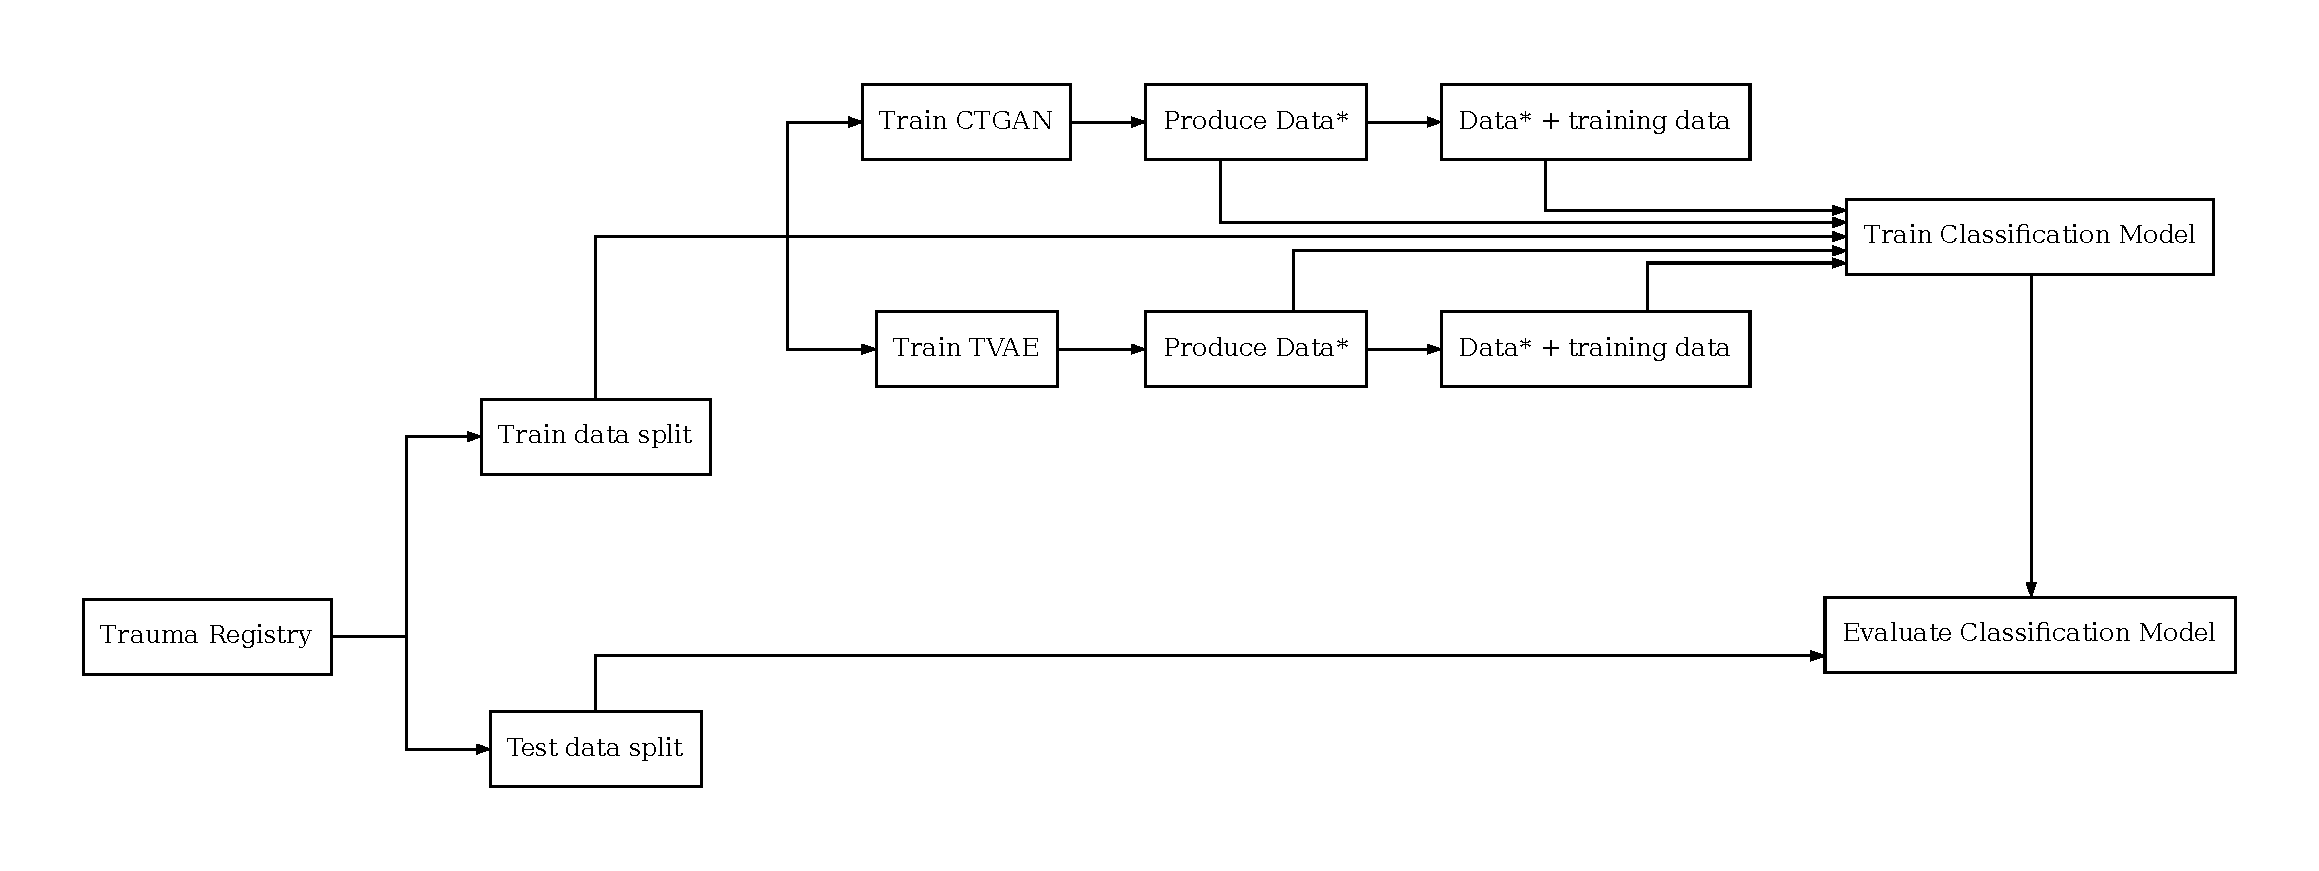
\includegraphics[width=\textwidth]{figures/model_flowchart.pdf}
    \caption{\textbf{Flowchart describing the process of evaluating the synthesising models.} Process is replicated for each classification model and resample. Each arrow to "Train Classification Model" indicates an individual and separated training/evaluation cycle from the other data inputs.\\
        *Synthetic training data output by a data synthesising model.\\
        \textit{Definition of abbreviations:} CTGAN = Conditional tabular generative adversarial network; TVAE = Triplet based variational autoencoder.}
    \label{fig:modelflowchart}
\end{figure}

The performance of the models was assessed on the test split from each resample and compared using \acrshort{auc}. The performance of a classification model was compared both to models within the same data group and to models in different data groups.

Descriptive statistics, including mean, \acrfull{sd}, median, minimum, and maximum for continuous and ordinal features, and prevalence for categorical features, were calculated. The missing prevalence for all features were calculated. Descriptive statistics were computed for both the baseline and synthetic datasets and grouped by: overall, \acrshort{ofi} positive, and \acrshort{ofi} negative. Descriptive statistics for patient demographic and clinical characteristics variables were chosen based on previously chosen variables that are important for \acrshort{ofi} detection \cite{attergrim_predicting_2023}.

\subsection{Ethical Considerations}
The group under investigation in this study, trauma patients, can be considered a vulnerable population due to the severe outcomes that often result from major trauma, such as disability and death. Thus, special consideration must be given to the ethics of conducting this study. It is important to note that only anonymous registry data was used in this study, and no identifiable personal data was accessible by the authors or the \acrshort{ml} models, this is one of the important measurements taken to reduce possible ethical complications.

In terms of autonomy and non-maleficence, no interventions were made that could potentially harm the patients. The registry on which this study was based, \acrshort{swetrau}, operates under the assumption of presumed consent, meaning that if a patient does not explicitly opt out of being included in the registry, it is assumed that they have consented to participate. While this study poses almost no risk of harm to the study population, the absence of sensitive personal data also reduces the risk of stigmatising a particular group.

The study aligns with the principle of beneficence, as its purpose is to improve clinical models for detecting \acrshortpl{ofi} and improve patient care in the long run. The study provides valuable insights into methods to improve the performance of \acrshort{ml} models in this area.

The ethical considerations associated with synthesising personal data warrant further discussion. If it were possible to generate 100\% anonymous synthesised data, would the same ethical principles apply? Since the synthesised data does not represent actual patients, it is difficult to consider autonomy and justice in this context. However, conducting epidemiological studies on randomly generated or simulated data is typically done without much ethical consideration. There must be a consensus on these ethical considerations before synthesising models can produce highly accurate synthetic data.

In conclusion, the benefits of this study, as measured against the four principles of Beauchamp and Childress (autonomy, non-maleficence, descence, and justice), outweigh the potential risks. The study was approved by the Stockholm Research Ethics Review Board (permits 2021-02541 and 2021-03531).

\section{Results}
\subsection{Patient Characteristics}

Between 2014 and 2021, a population of \num{12107} trauma patients was identified, of which \num{6314} were excluded due to not being screened for an \acrshort{ofi} by either audit filters or individual review. None of the patients were excluded for being under the age of 15. Therefore, a total of \num{5793} patients were deemed eligible and included in the study. Among these cases, \num{5453} patients had no \acrshort{ofi}, while \num{340} patients were diagnosed with at least one \acrshort{ofi}. A summarised graph of the inclusion and exclusion criteria, as well as the process to an \acrshort{ofi}, can be seen in \Cref{fig:flowchart}.

\begin{figure}
    \centering
    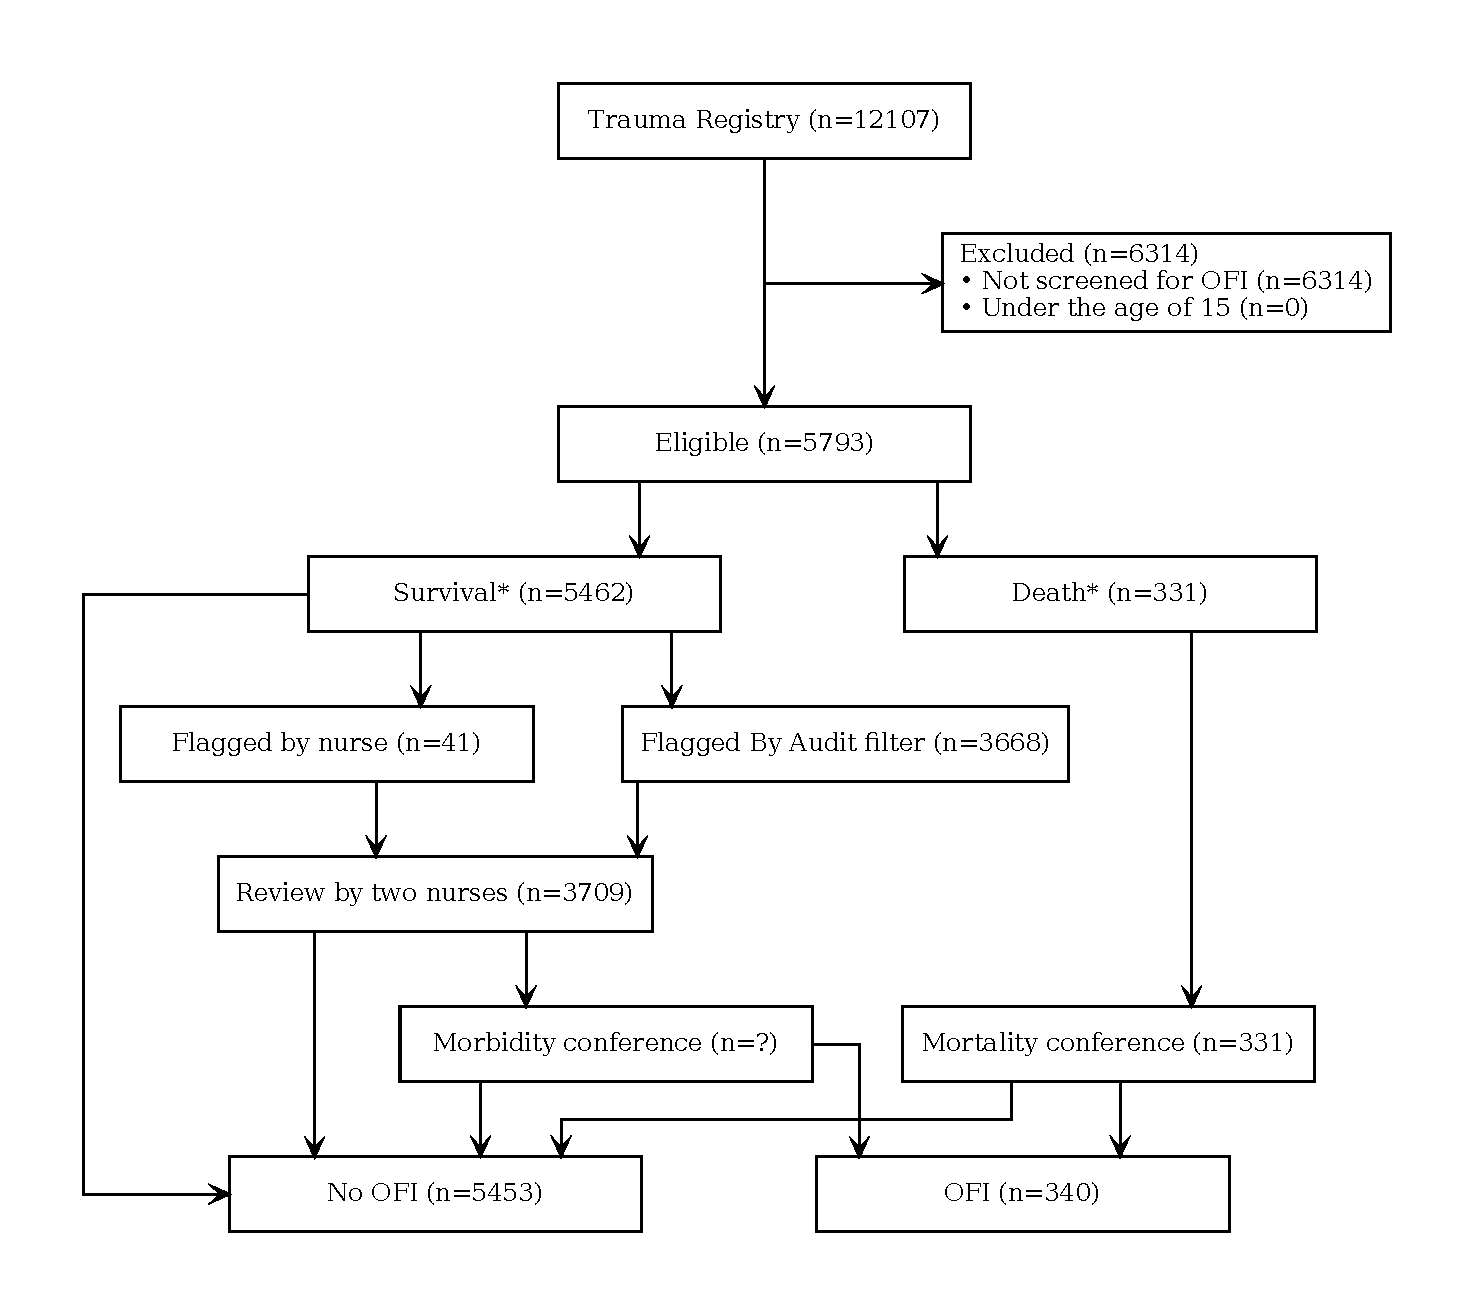
\includegraphics[width=0.6\textwidth]{figures/flowchart.pdf}
    \caption{\textbf{Flowchart describing the exclusions made and including the process to determine a case with \acrshort{ofi}.} The amount of patient cases brought up at a morbidity conference is unknown in the current dataset.\\
        *Defined at 30-days post trauma.\\
        \textit{Definition of abbreviations:} OFI = opportunity for improvement.}
    \label{fig:flowchart}
\end{figure}

Selected patient characteristics are summarised in \Cref{tab:tableone}. The trauma group as a whole had a mean age of 46 (\acrshort{sd}: 21), while the \acrshort{ofi} and \acrshort{ofi}-negative subgroups had a mean age of 50 (\acrshort{sd}: 22) and 45 (\acrshort{sd}: 21), respectively. The majority of patients were male ($n = $ \num{3509}, 61\%), and the overall group had a mortality rate of 6\% ($n = $ \num{331}). The \acrshort{ofi} group had a higher mean \acrshort{iss} (18 [\acrshort{sd}: 10] vs 10 [\acrshort{sd}: 11]) and were admitted to the intensive care unit more frequently (30\% [$n = $ \num{286}] vs 14\% [$n = $ \num{761}]). Data for emergency procedures were less missing in the \acrshort{ofi} subgroup, with 54\% ($n = $ 182) of records missing data compared to 82\% ($n = $ \num{4452}) in the \acrshort{ofi}-negative group. Furthermore, the "other" emergency procedure was more common in the \acrshort{ofi} group (26\% [$n = $ \num{88}] vs 13\% [$n = $ \num{699}]).

\begin{table}[p]
    \centering
    \renewcommand{\arraystretch}{0.9}
    \caption{\textbf{Selected patient demographic and clinical characteristics}. Subdivided by \acrshort{ofi} outcome for baseline data.}
    \label{tab:tableone}
    \scalebox{0.7}{
        \begin{tabular}{lccc}
            \toprule
                                                          & \textbf{Overall}  & \textbf{No OFI}   & \textbf{OFI}     \\
            \midrule
                                                          & $n=5793$          & $n=5453$          & $n=340$          \\
            \textbf{Age}                                  &                   &                   &                  \\
            \hspace{3mm}Mean (SD)                         & 46 (21)           & 45 (21)           & 50 (22)          \\
            \hspace{3mm}Median [Min, Max]                 & 43 [15, 100]      & 43 [15, 100]      & 50 [15, 97]      \\
            \hspace{3mm}Missing                           & 651 (11\%)        & 617 (11\%)        & 34 (10\%)        \\
            \textbf{Gender}                               &                   &                   &                  \\
            \hspace{3mm}Male                              & 3509 (61\%)       & 3293 (60\%)       & 216 (64\%)       \\
            \hspace{3mm}Female                            & 1633 (28\%)       & 1543 (28\%)       & 90 (26\%)        \\
            \hspace{3mm}Missing                           & 651 (11\%)        & 617 (11\%)        & 34 (10\%)        \\
            \textbf{Dead at 30 days}                      &                   &                   &                  \\
            \hspace{3mm}No                                & 4809 (83\%)       & 4523 (83\%)       & 286 (84\%)       \\
            \hspace{3mm}Yes                               & 331 (6\%)         & 311 (6\%)         & 20 (6\%)         \\
            \hspace{3mm}Missing                           & 653 (11\%)        & 619 (11\%)        & 34 (10\%)        \\
            \textbf{Highest level of care}                &                   &                   &                  \\
            \hspace{3mm}Intensive care unit               & 863 (15\%)        & 761 (14\%)        & 102 (30\%)       \\
            \hspace{3mm}General ward                      & 2002 (35\%)       & 1933 (35\%)       & 69 (20\%)        \\
            \hspace{3mm}Surgical ward                     & 945 (16\%)        & 852 (16\%)        & 93 (27\%)        \\
            \hspace{3mm}ED                                & 1120 (19\%)       & 1106 (20\%)       & 14 (4\%)         \\
            \hspace{3mm}Specialist/Intermediate ward      & 212 (4\%)         & 184 (3\%)         & 28 (8\%)         \\
            \hspace{3mm}Missing                           & 651 (11\%)        & 617 (11\%)        & 34 (10\%)        \\
            \textbf{Injury severity score}                &                   &                   &                  \\
            \hspace{3mm}Mean (SD)                         & 10 (11)           & 10 (11)           & 18 (10)          \\
            \hspace{3mm}Median [Min, Max]                 & 8 [0, 75]         & 5 [0, 75]         & 17 [0, 59]       \\
            \hspace{3mm}Missing                           & 653 (11\%)        & 619 (11\%)        & 34 (10\%)        \\
            \textbf{ED Respiratory Rate}                  &                   &                   &                  \\
            \hspace{3mm}Mean (SD)                         & 23 (20)           & 23 (20)           & 24 (21)          \\
            \hspace{3mm}Median [Min, Max]                 & 18 [0, 99]        & 18 [0, 99]        & 18 [0, 99]       \\
            \hspace{3mm}Missing                           & 683 (12\%)        & 644 (12\%)        & 39 (11\%)        \\
            \textbf{ED Systolic blood pressure}           &                   &                   &                  \\
            \hspace{3mm}Mean (SD)                         & 136 (28)          & 136 (28)          & 135 (31)         \\
            \hspace{3mm}Median [Min, Max]                 & 135 [0, 285]      & 135 [0, 285]      & 135 [0, 237]     \\
            \hspace{3mm}Missing                           & 660 (11\%)        & 626 (11\%)        & 34 (10\%)        \\
            \textbf{ED GCS}                               &                   &                   &                  \\
            \hspace{3mm}Mean (SD)                         & 14 (2)            & 14 (2)            & 14 (2)           \\
            \hspace{3mm}Median [Min, Max]                 & 15 [3, 15]        & 15 [3, 15]        & 15 [3, 15]       \\
            \hspace{3mm}Missing                           & 1008 (17\%)       & 950 (17\%)        & 58 (17\%)        \\
            \textbf{Time to first CT}                     &                   &                   &                  \\
            \hspace{3mm}Mean (SD)                         & 75 (137)          & 74 (137)          & 82 (139)         \\
            \hspace{3mm}Median [Min, Max]                 & 35 [0, 1415]      & 35 [0, 1415]      & 43 [6, 1339]     \\
            \hspace{3mm}Missing                           & 1206 (21\%)       & 1147 (21\%)       & 59 (17\%)        \\
            \textbf{Time to definitive treatment}         &                   &                   &                  \\
            \hspace{3mm}Mean (SD)                         & 263 (354)         & 260 (358)         & 278 (328)        \\
            \hspace{3mm}Median [Min, Max]                 & 110 [0, 2036]     & 104 [0, 2036]     & 154 [9, 1420]    \\
            \hspace{3mm}Missing                           & 4635 (80\%)       & 4453 (82\%)       & 182 (54\%)       \\
            \textbf{Intubated}                            &                   &                   &                  \\
            \hspace{3mm}No                                & 5285 (91\%)       & 4997 (92\%)       & 288 (85\%)       \\
            \hspace{3mm}Yes                               & 508 (9\%)         & 456 (8\%)         & 52 (15\%)        \\
            \hspace{3mm}Missing                           & 0 (0\%)           & 0 (0\%)           & 0 (0\%)          \\
            \textbf{Emergency procedure}                  &                   &                   &                  \\
            \hspace{3mm}Laparotomy                        & 114 (2\%)         & 100 (2\%)         & 14 (4\%)         \\
            \hspace{3mm}Craniotomy                        & 131 (2\%)         & 111 (2\%)         & 20 (6\%)         \\
            \hspace{3mm}Other                             & 787 (14\%)        & 699 (13\%)        & 88 (26\%)        \\
            \hspace{3mm}Radiological intervention         & 51 (\textless1\%) & 29 (\textless1\%) & 22 (6\%)         \\
            \hspace{3mm}Thoracotomy                       & 18 (\textless1\%) & 17 (\textless1\%) & 1 (\textless1\%) \\
            \hspace{3mm}Intracranial pressure measurement & 34 (\textless1\%) & 28 (\textless1\%) & 6 (2\%)          \\
            \hspace{3mm}Revascularisation                 & 22 (\textless1\%) & 15 (\textless1\%) & 7 (2\%)          \\
            \hspace{3mm}Pelvis packing                    & 2 (\textless1\%)  & 2 (\textless1\%)  & 0 (0\%)          \\
            \hspace{3mm}Missing                           & 4634 (80\%)       & 4452 (82\%)       & 182 (54\%)       \\
            \bottomrule
        \end{tabular}
    }
    \caption*{\small Time to first CT and Time to definitive treatment are measured in minutes from arrival at the hospital.\\
        \textit{Definition of abbreviations:} OFI = Opportunity for Improvement; ED = Emergency Department; GCS = Glascow Coma Scale.}
\end{table}

Selected patient characteristics for the data produced by the synthesising models for the first resample are presented in \Cref{tab:tableonectgan,tab:tableonetvae} in the appendix. The \acrshort{tvae} dataset produced fewer \acrshort{ofi} cases ($n=101$) than both the baseline and \acrshort{ctgan} ($n=500$). The overall mean age was 56 (\acrshort{sd}: 23) and 51 (\acrshort{sd}: 26) for \acrshort{ctgan} and \acrshort{tvae}, respectively. The \acrshort{ctgan} dataset produced more missing data, with the most missing data found in the Emergency procedure predictor with 87\% (76\% in the \acrshort{tvae} group) and the least missing data with 0\% in the Intubated predictor (0\% in the \acrshort{tvae} group). Excluding the Intubated predictor, the predictors with the lowest number of missing values were Age, Gender, Dead at 30 days, Highest level of care, and Emergency department GCS with 36\% of data points missing values in the \acrshort{ctgan} group. The same predictors in the \acrshort{tvae} group had all missing values in 6\% of data points. The mean Emergency Department Glasgow Coma Scale was 21 and 20 for \acrshort{ctgan} and \acrshort{tvae}, respectively. Additionally, the \acrshort{tvae} group did not produce "Laparotomy", "Thoracotomy", and "Pelvis packing" for Emergency procedure.

\subsection{Model Performance}
The overall best data group was the baseline group with 6 out of 8 models scoring significantly their best \acrshort{auc} score in that group. The $k$-nearest neighbour model scored its best \acrshort{auc} in the \acrshort{ctgan} + baseline group. However, this performance improvement was insignificant with a mean \acrshort{auc} of 0.717 (0.711, 0.722) in the \acrshort{ctgan} + baseline group and an \acrshort{auc} of 0.715 (0.71, 0.721) in the baseline group.

The random forest model achieved the best overall \acrshort{auc} result out of all classification models in all data groups, it scored an \acrshort{auc} of 0.792 (0.787, 0.797) in the baseline group, this was not significant compared to the \acrshort{ctgan} + baseline group (\acrshort{auc}: 0.784 [0.779, 0.788]). The second best model, with an overlapping \acrshort{ci} to the baseline random forest model, was CatBoost (\acrshort{auc}: 0.789 [0.784, 0.794]). The worst performing model was the support vector machine, scoring its best \acrshort{auc} in the baseline group (\acrshort{auc}: 0.675 [0.668, 0.681]). All synthesising models generated data that achieved significant discrimination result (AUC $> 0.5$) apart from \acrshort{ctgan}, where the support vector machine could not achieve a significant discriminatory \acrshort{auc} (\acrshort{auc}: 0.501 [0.489, 0.514]). Additionally, when adding the \acrshort{ctgan} and baseline data, the support vector machine scored the worst overall score (\acrshort{auc}: 0.449 [0.424, 0.474]). See \Cref{tab:modelperf} for \acrshort{auc} metrics for all classification models in each data group and corresponding \acrshortpl{ci}.


\begin{table}
    \centering
    \renewcommand{\arraystretch}{0.8}
    \caption{\textbf{\acrshort{auc} performance in predicting \acrshort{ofi}.} The average \acrshort{auc} (95\% \acrshort{ci}) for classification models in each data group. The best performing data group for each classification model is displayed in bold.}
    \label{tab:modelperf}
    \scalebox{0.75}{
        \begin{tabular}{lccccc}
            \toprule
            \textbf{Model}                       & \textbf{Baseline}       & \textbf{CTGAN} & \textbf{TVAE}  & \textbf{CTGAN + Baseline} & \textbf{TVAE + Baseline} \\
            \midrule
            \multirow{2}{*}{CatBoost}            & \textbf{0.789}          & 0.565          & 0.637          & 0.777                     & 0.776                    \\
                                                 & \textbf{(0.784, 0.794)} & (0.551, 0.579) & (0.615, 0.659) & (0.772, 0.782)            & (0.771, 0.781)           \\[0.5em]
            \multirow{2}{*}{Extra Trees}         & \textbf{0.776}          & 0.599          & 0.604          & 0.762                     & 0.765                    \\
                                                 & \textbf{(0.771, 0.781)} & (0.586, 0.611) & (0.585, 0.622) & (0.757, 0.768)            & (0.76, 0.77)             \\[0.5em]
            \multirow{2}{*}{k-NN}                & 0.715                   & 0.533          & 0.527          & \textbf{0.717}            & 0.689                    \\
                                                 & (0.71, 0.721)           & (0.52, 0.545)  & (0.521, 0.533) & \textbf{(0.711, 0.722)}   & (0.682, 0.695)           \\[0.5em]
            \multirow{2}{*}{LightGBM}            & \textbf{0.783}          & 0.549          & 0.604          & 0.772                     & 0.772                    \\
                                                 & \textbf{(0.778, 0.788)} & (0.537, 0.56)  & (0.587, 0.62)  & (0.767, 0.776)            & (0.766, 0.777)           \\[0.5em]
            \multirow{2}{*}{Logistic Regression} & \textbf{0.764}          & 0.595          & 0.618          & 0.748                     & 0.751                    \\
                                                 & \textbf{(0.759, 0.769)} & (0.58, 0.609)  & (0.592, 0.643) & (0.742, 0.754)            & (0.745, 0.756)           \\[0.5em]
            \multirow{2}{*}{Random forest}       & \textbf{0.792}          & 0.629          & 0.619          & 0.784                     & 0.777                    \\
                                                 & \textbf{(0.787, 0.797)} & (0.619, 0.639) & (0.603, 0.636) & (0.779, 0.788)            & (0.772, 0.783)           \\[0.5em]
            \multirow{2}{*}{SVM}                 & \textbf{0.675}          & 0.501          & 0.616          & 0.449                     & 0.648                    \\
                                                 & \textbf{(0.668, 0.681)} & (0.489, 0.514) & (0.593, 0.64)  & (0.424, 0.474)            & (0.641, 0.655)           \\[0.5em]
            \multirow{2}{*}{XGBoost}             & \textbf{0.771}          & 0.573          & 0.629          & 0.749                     & 0.745                    \\
                                                 & \textbf{(0.767, 0.776)} & (0.559, 0.588) & (0.602, 0.657) & (0.743, 0.754)            & (0.739, 0.751)           \\
            \bottomrule
        \end{tabular}

    }
    \caption*{\small \textit{Definition of abbreviations:} AUC = \acrlong{auc}; CI = \acrlong{ci}; k-NN = $k$-nearest neighbour; OFI = \acrlong{ofi}; SVM = support vector machine.}
\end{table}

The average receiver operating characteristic curve for classification models within a data group is presented in \Cref{fig:roc}. The baseline, \acrshort{ctgan} + baseline, and \acrshort{tvae} + baseline data groups exhibit similar receiver operating characteristic curves and \acrshort{auc} scores. The baseline group demonstrated the best overall average \acrshort{auc} of 0.753. In comparison, the \acrshort{ctgan} data group demonstrated better performance in the high false positive and true positive rate range than the \acrshort{tvae} data group, but lower performance in the low false positive and true positive rate range. This was also seen in the curve when the baseline data was added to each group. The \acrshort{ctgan} data group performed the worst, with an average \acrshort{auc} of 0.555.

\begin{figure}
    \centering
    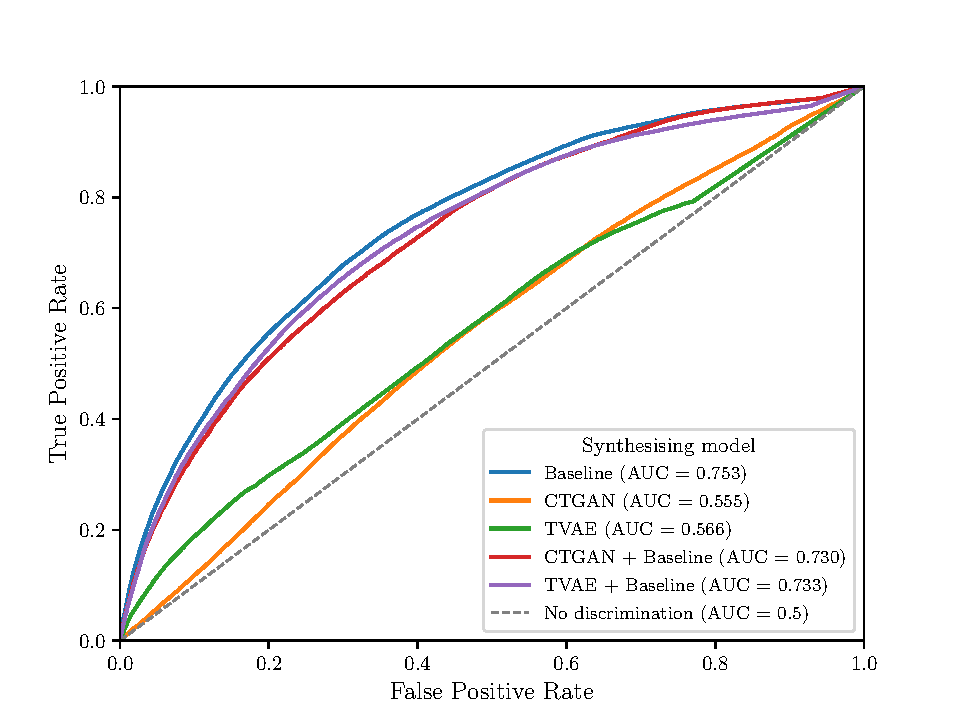
\includegraphics[width=0.85\textwidth]{figures/roc.pdf}
    \caption{\textbf{Average receiver operating characteristic curve for classification models within a data group.} Each data group curve was calculated by taking the average curve for all classification within a data group. \\
        \textit{Definition of abbreviations:} AUC = \Acrlong{auc}; CTGAN = \Acrlong{ctgan}; TVAE = \Acrlong{tvae}.}
    \label{fig:roc}
\end{figure}

\newpage

\section{Discussion}
The aim of this study was to evaluate the effectiveness of generating synthetic data in a trauma setting using a \acrshort{gan} and \acrshort{vae} in improving \acrshort{ofi} prediction models. The generated data from the \acrshort{gan} and \acrshort{vae} tested resulted in significantly worse performance in predicting \acrshortpl{ofi} with classification models compared models trained with the baseline data. The average performance loss compared to the baseline data in terms of \acrshort{auc} was 0.198 and 0.187 for the \acrshort{gan} and \acrshort{vae} respectively. The results display the current infeasibility of generating synthetic data to improve \acrshort{ofi} prediction models in a trauma setting.

The \acrshort{vae} based model implemented in this study showed an overall better performance in generating data than the \acrshort{gan} based model. Four of the classification models achieved significantly better performance using the \acrshort{vae} data compared to the \acrshort{gan} data, the remaining four models were non-inferior. However, the average \acrshort{auc} difference for the groups as a whole was minimal, 0.566 vs 0.555 for the \acrshort{vae} and \acrshort{gan} respectively. This may indicate that generating synthetic data in this context is a difficult task rather than the fault of the specific methods.

An interesting observation is that when combining the \acrshort{vae} or \acrshort{gan} data with the baseline data, the difference from the baseline data, though significant, was minimal. The average difference of the three best performing classification models (CatBoost, LightGBM, random forest) baseline performance versus the \acrshort{gan} + baseline performance was 0.01. For \acrshort{vae}, it was also 0.01. Despite the baseline and synthetic datasets being equally large, the classification models were barely affected by the poor synthetic data. The test data used in each resample split was not presented to the models until evaluation, meaning that the classification models learnt the most important features in the combined data despite the noise added by the synthetic data.

This hints that an improvement of the synthetic data quality might improve the performance of classification models trained on both baseline + synthetic data compared to only baseline. This, despite the synthetic data in of itself not improving the performance of the classification models. It is conceivable that this is due to the synthetic data being produced not including data points close to the ones in the baseline data and instead more edge cases. Resulting in that classification models trained on only synthetic data performs poorly, due to only learning edge cases, but models trained on a combination results in more robust models, due to learning both the bulk data and edge cases.

The baseline results exhibit similarities to those reported by Attergrim et al. \cite{attergrim_predicting_2023}, who found that LightGBM and random forest were the best-performing models. Hernandez et al. \cite{hernandez_synthetic_2022} reported varied performance of synthetic data generation using \acrlongpl{gan} in different medical contexts. One conclusion drawn by Hernandez and colleagues was that the existing \acrlong{gan}-based approaches are not generalisable to all types of tabular data. This is further supported by the present study where the tested \acrshort{ctgan} displayed poor performance compared to the baseline. Abedi et al. \cite{abedi_gan-based_2022} investigated how the size of the training data affected the performance of classification models trained with synthetic data. For certain training data sizes, the results were similar to those found in the current study. This may indicate that, for the time being, there is not enough data to use the methods tested.

The quality of the data generated by the various predictors for the synthetic datasets varies. For example, both synthesisers erroneously produced Glasgow coma scale scores over 15. The \acrlong{tvae} model's dataset has overall means and incidences that are closer to those of the baseline dataset. However, the \acrshort{tvae} model seems to produce a less varied \acrshort{ofi} positive group. As shown in \Cref{tab:tableonetvae}, \acrshort{tvae} for \acrshort{ofi} positive cases ($n=101$) produced 100\% male, 95\% not dead at 30 days, and 94\% with the intensive care unit as the highest level of care. Compared with the baseline characteristics in \Cref{tab:tableone}, the incidence for the same predictors were 64\%, 84\%, and 30\%, respectively. When it comes to categorical predictors, the \acrshort{ctgan} model's data was more aligned with the baseline characteristics.

Finally, despite the results of the current study, if it were possible to generate synthetic data to improve \acrshort{ml} prediction model performance, it would most likely be better to use the synthesising model directly as a prediction model. Synthetic data generators cannot add more information than what was already in the baseline data; they learn features and correlations in the baseline data and use them to generate data. Similarly, classification models learn features and correlations in the baseline data but use them to predict a class instead. Therefore, to produce quality data that a classification model can learn from, the synthetic data generator has to learn features and correlations in the baseline dataset better than what the classification models can. If we were to change the synthetic data generator's task from generating data to classifying data, we could expect the same, if not better, performance than the previously used classification model. This has been explored with using \acrshortpl{gan} for classification by Israel et al. \cite{israel_generative_2017}.

\subsection{Strengths and Limitations}
There are several strengths to the present study. Firstly, the code used to develop the models was developed without running it on the true data until validation time. Secondly, the methodology uses a robust way of validation. Resampling using 100 resamples allows for virtual simulation of rerunning the experiment 100 times, providing the ability to calculate confidence intervals to ensure statistical significance between models. Thirdly, the classification models are based on an already validated methodology using state-of-the-art models. This means that we can compare our baseline results to previous results to ensure that the current models have been applied correctly.

However, there are limitations to the study. Firstly, the sample size is relatively small ($n = 5793$). This can be compared with the original implementation studies that use at least tens of thousands of data points, and in many cases, much more \cite{xu_modeling_2019,karras_training_2020}. Furthermore, only two synthetic data generation models were tested, whereas there exist many more types of models, some more specific for medical data \cite{hernandez_synthetic_2022}.

\subsection{Practical Applications}
The present study, despite the inferior results of the tested synthetic data generation models, has developed a framework that enables the validation of synthetic data generation methods using machine learning models for predicting ocular foreign bodies (OFI). This modular framework facilitates the testing and validation of further synthesising models with minimal effort. Moreover, the framework is extensible in terms of the classification models, allowing for the addition of more.

The implication of this development is that synthetic data generation methods can be rapidly tested and validated. If, or when, a synthetic data generation method is validated that can generate accurate synthetic trauma datasets, these could theoretically be distributed to the wider scientific community. This could have a significant impact, particularly in furthering the possibility of open and reproducible science in medicine. It could also lead to easier distribution of data, facilitating simpler methods for external validation. Finally, it allows for the possibility that several research groups can work on the same problem.

However, ethical questions have to be considered. For instance, whether the synthetic dataset requires the same ethical considerations as the true data. Another issue is ensuring that the synthetic data represents the population as a whole. As evidenced by the TVAE-generated data, the OFI positive population was predominantly male. This could result in gender, age, or other socio-demographic factors being over or under-represented in the synthetic datasets. It is crucial to ensure that future synthetic datasets do not suffer from this issue to ensure health equity.

\subsection{Future Studies}
Future studies should aim to investigate whether other synthetic data generation techniques can provide beneficial results, building on the framework developed in the present study. This could help determine whether synthetic data generation is possible for smaller trauma datasets.

In addition, it is important to implement supplementary methods for evaluating the quality and privacy of the generated datasets. The current method only tests quality in terms of \acrshort{ofi} prediction, but there are many other correlations that need to be assessed. Furthermore, the actual performance of generating anonymised datasets was not tested. Both these questions could be explored by implementing the multifaceted benchmarking framework for synthetic electronic health records introduced by Yan et al. \cite{yan_multifaceted_2022}.

\section{Conclusions}
The present study suggests that the current \acrshort{gan} and \acrshort{vae}-based methods are unsuitable for generating synthetic data for \acrshort{ofi} prediction in trauma patient care. The performance of the \acrshort{ml} models trained on data synthesised by the \acrshort{ctgan} and \acrshort{tvae} models in predicting \acrshortpl{ofi} in trauma patient care was significantly worse then models trained on baseline data. However, further research is required to determine whether other \acrshort{gan}-based models, with additional adjustments, could produce an acceptable performance.

\newpage

\singlespacing

\printbibliography

\newpage

\begin{appendices}
    \setcounter{table}{0}
    \renewcommand{\thetable}{A\arabic{table}}

    \setcounter{figure}{0}
    \renewcommand{\thefigure}{A\arabic{figure}}

    \setcounter{secnumdepth}{1}

    \section{Tables}
    \begin{table}[h]
        \centering
        \renewcommand{\arraystretch}{1.2}

        \caption{\textbf{All the currently used audit filters at Karolinska University Hospital.}}
        \label{tab:auditfilters}

        \begin{tabular}{@{}|p{0.85\linewidth}|@{}}
            \hline
            \multicolumn{1}{|c|}{\textbf{Audit filter}}                                                \\\hline
            Systolic blood pressure less than 90                                                       \\\hline
            Glasgow coma scale less than 9 and not intubated                                           \\\hline
            Injury severity score greater than 15 but not admitted to the intensive care unit          \\\hline
            Time to acute intervention more than 60 minutes from arrival to hospital                   \\\hline
            Time to computed tomography more than 30 minutes from arrival to hospital                  \\\hline
            No anticoagulant therapy within 72 hours after traumatic brain injury                      \\\hline
            The presence of cardio-pulmonary resuscitation with thoracotomy                            \\\hline
            The presence of a liver or spleen injury                                                   \\\hline
            Massive transfusion, defined as 10 or more units of packed red blood cells within 24 hours \\\hline
            Other non-defined reason found by first reviewing nurse                                    \\\hline
        \end{tabular}
    \end{table}


    \renewcommand*{\arraystretch}{1.2}
    \begin{longtable}[c]{@{}|l|p{0.55\linewidth}|@{}}
        \caption{\textbf{Predictors used in the development of the \acrlong{ofi} classification and synthesising models.}}%
        \label{tab:predictors}                                                                                          \\
        \hline
        \multicolumn{1}{|c|}{\textbf{SweTrau code}} & \multicolumn{1}{|c|}{\textbf{Description}}                        \\\hline
        \endfirsthead
        %
        \endhead
        %
        AlarmRePrioritised                          & Reprioritisation of trauma code                                   \\\hline
        FirstTraumaDT\_NotDone                      & Trauma CT not done                                                \\\hline
        ISS                                         & Injury Severity Score                                             \\\hline
        NumberOfActions                             & Number of Actions done                                            \\\hline
        NumberOfInjuries                            & Number of injuries                                                \\\hline
        TraumaAlarmAtHospital                       & Type of trauma code criteria                                      \\\hline
        TraumaAlarmCriteria                         & Trauma code at hospital                                           \\\hline
        dt\_alarm\_hosp                             & DT alarm to ED                                                    \\\hline
        dt\_alarm\_scene                            & DT alarm to arrival at scene                                      \\\hline
        dt\_ed\_emerg\_proc                         & DT arrival at ED to emergency procedure                           \\\hline
        dt\_ed\_first\_ct                           & DT arrival at ED to first CT                                      \\\hline
        dt\_ed\_norm\_be                            & DT arrival ED to normalised base excess                           \\\hline
        ed\_be\_art                                 & First base excess at the ED                                       \\\hline
        ed\_be\_art\_NotDone                        & Base excess not taken at ED                                       \\\hline
        ed\_emerg\_proc                             & Emergency procedure at ED                                         \\\hline
        ed\_emerg\_proc\_other                      & Other emergency procedure at ED                                   \\\hline
        ed\_gcs\_motor                              & Motor response according to GCS at ED                             \\\hline
        ed\_gcs\_sum                                & GCS score at ED                                                   \\\hline
        ed\_inr                                     & First Prothrombin time (international normalise ratio)            \\\hline
        ed\_inr\_NotDone                            & Prothrombin time (international normalised ratio) not taken at ED \\\hline
        ed\_intub\_type                             & Intubation type at ED                                             \\\hline
        ed\_intubated                               & Was intubated at ED                                               \\\hline
        ed\_rr\_value                               & Respiratory rate at ED                                            \\\hline
        ed\_sbp\_value                              & Systolic blood pressure at ED                                     \\\hline
        ed\_tta                                     & Trauma team activated                                             \\\hline
        hosp\_dischg\_dest                          & Discharge destination                                             \\\hline
        hosp\_los\_days                             & Total admittance days at hospital                                 \\\hline
        hosp\_vent\_days                            & Total amount of days in a ventilator                              \\\hline
        host\_care\_level                           & Highest level of care                                             \\\hline
        host\_transfered                            & Transferred from/to another hospital                              \\\hline
        host\_vent\_days\_NotDone                   & No days spent on a ventilator                                     \\\hline
        inj\_dominant                               & Dominant type of injury                                           \\\hline
        inj\_intention                              & Injury intention                                                  \\\hline
        inj\_mechanism                              & Dominant injury mechanism                                         \\\hline
        iva\_dagar\_n                               & Total amount of days in the intensive care unit                   \\\hline
        iva\_vardtillfallen\_n                      & Amount of times admitted to the intensive care unit               \\\hline
        pre\_card\_arrest                           & PH cardiac arrest                                                 \\\hline
        pre\_gcs\_motor                             & PH motor response according to GCS                                \\\hline
        pre\_gcs\_sum                               & PH GCS score                                                      \\\hline
        pre\_intub\_type                            & Type of intubation PH                                             \\\hline
        pre\_intubated                              & Was intubated PH                                                  \\\hline
        pre\_provided                               & Level of care given PH                                            \\\hline
        pre\_rr\_value                              & PH Respiratory rate                                               \\\hline
        pre\_sbp\_value                             & PH Systolic blood pressure                                        \\\hline
        pre\_transport                              & Transport type PH                                                 \\\hline
        pt\_Gender                                  & Gender                                                            \\\hline
        pt\_age\_yrs                                & Patient age                                                       \\\hline
        pt\_asa\_preinjury                          & American Society of Anesthesiologists Class pre-injury            \\\hline
        res\_gos\_dischg                            & Glascow outcome score at discharge                                \\\hline
        res\_survival                               & Mortality                                                         \\\hline
        \caption*{\small \textit{Definition of abbreviations:} CT = Computer Tomography; DT = Delta Time; ED = Emergency department; GCS = Glascow Coma Scale; PH = Pre-hospital.}%
    \end{longtable}

    \begin{table}[t!]
        \centering
        \renewcommand{\arraystretch}{0.9}
        \caption{\textbf{Selected patient demographic and clinical characteristics}. Subdivided by \acrshort{ofi} outcome for \acrshort{ctgan} data.}
        \label{tab:tableonectgan}
        \scalebox{0.7}{
            \begin{tabular}{lccc}
                \toprule
                                                              & \textbf{Overall}  & \textbf{No OFI}   & \textbf{OFI}     \\
                \midrule
                                                              & $n=5793$          & $n=5293$          & $n=500$          \\
                \textbf{Age}                                  &                   &                   &                  \\
                \hspace{3mm}Mean (SD)                         & 56 (23)           & 56 (23)           & 55 (23)          \\
                \hspace{3mm}Median [Min, Max]                 & 56 [15, 100]      & 56 [15, 100]      & 53 [15, 100]     \\
                \hspace{3mm}Missing                           & 2112 (36\%)       & 1847 (35\%)       & 265 (53\%)       \\
                \textbf{Gender}                               &                   &                   &                  \\
                \hspace{3mm}Female                            & 1566 (27\%)       & 1465 (28\%)       & 101 (20\%)       \\
                \hspace{3mm}Male                              & 2122 (37\%)       & 1988 (38\%)       & 134 (27\%)       \\
                \hspace{3mm}Missing                           & 2105 (36\%)       & 1840 (35\%)       & 265 (53\%)       \\
                \textbf{Dead at 30 days}                      &                   &                   &                  \\
                \hspace{3mm}No                                & 3577 (62\%)       & 3350 (63\%)       & 227 (45\%)       \\
                \hspace{3mm}Yes                               & 121 (2\%)         & 113 (2\%)         & 8 (2\%)          \\
                \hspace{3mm}Missing                           & 2095 (36\%)       & 1830 (35\%)       & 265 (53\%)       \\
                \textbf{Highest level of care}                &                   &                   &                  \\
                \hspace{3mm}General ward                      & 2041 (35\%)       & 1928 (36\%)       & 113 (23\%)       \\
                \hspace{3mm}Intensive care unit               & 842 (15\%)        & 780 (15\%)        & 62 (12\%)        \\
                \hspace{3mm}ED                                & 410 (7\%)         & 385 (7\%)         & 25 (5\%)         \\
                \hspace{3mm}Surgical ward                     & 334 (6\%)         & 305 (6\%)         & 29 (6\%)         \\
                \hspace{3mm}Specialist/Intermediate ward      & 67 (1\%)          & 62 (1\%)          & 5 (1\%)          \\
                \hspace{3mm}Missing                           & 2099 (36\%)       & 1833 (35\%)       & 266 (53\%)       \\
                \textbf{Injury severity score}                &                   &                   &                  \\
                \hspace{3mm}Mean (SD)                         & 7 (9)             & 7 (9)             & 8 (9)            \\
                \hspace{3mm}Median [Min, Max]                 & 5 [0, 75]         & 5 [0, 75]         & 8 [0, 74]        \\
                \hspace{3mm}Missing                           & 2116 (37\%)       & 1851 (35\%)       & 265 (53\%)       \\
                \textbf{ED Respiratory Rate}                  &                   &                   &                  \\
                \hspace{3mm}Mean (SD)                         & 27 (24)           & 27 (23)           & 28 (24)          \\
                \hspace{3mm}Median [Min, Max]                 & 21 [4, 99]        & 21 [4, 99]        & 22 [6, 99]       \\
                \hspace{3mm}Missing                           & 2311 (40\%)       & 2025 (38\%)       & 286 (57\%)       \\
                \textbf{ED Systolic blood pressure}           &                   &                   &                  \\
                \hspace{3mm}Mean (SD)                         & 148 (36)          & 148 (36)          & 141 (35)         \\
                \hspace{3mm}Median [Min, Max]                 & 143 [0, 285]      & 143 [0, 285]      & 138 [0, 274]     \\
                \hspace{3mm}Missing                           & 2238 (39\%)       & 1960 (37\%)       & 278 (56\%)       \\
                \textbf{ED GCS}                               &                   &                   &                  \\
                \hspace{3mm}Mean (SD)                         & 21 (32)           & 21 (32)           & 22 (24)          \\
                \hspace{3mm}Median [Min, Max]                 & 15 [3, 999]       & 15 [3, 999]       & 15 [3, 121]      \\
                \hspace{3mm}Missing                           & 2102 (36\%)       & 1839 (35\%)       & 263 (53\%)       \\
                \textbf{Time to first CT}                     &                   &                   &                  \\
                \hspace{3mm}Mean (SD)                         & 51 (80)           & 50 (79)           & 58 (91)          \\
                \hspace{3mm}Median [Min, Max]                 & 29 [0, 1033]      & 29 [0, 1033]      & 34 [2, 750]      \\
                \hspace{3mm}Missing                           & 2477 (43\%)       & 2167 (41\%)       & 310 (62\%)       \\
                \textbf{Time to definitive treatment}         &                   &                   &                  \\
                \hspace{3mm}Mean (SD)                         & 314 (294)         & 317 (298)         & 285 (245)        \\
                \hspace{3mm}Median [Min, Max]                 & 267 [1, 1727]     & 267 [1, 1727]     & 266 [18, 1311]   \\
                \hspace{3mm}Missing                           & 4925 (85\%)       & 4490 (85\%)       & 435 (87\%)       \\
                \textbf{Intubated}                            &                   &                   &                  \\
                \hspace{3mm}No                                & 5490 (95\%)       & 5025 (95\%)       & 465 (93\%)       \\
                \hspace{3mm}Yes                               & 303 (5\%)         & 268 (5\%)         & 35 (7\%)         \\
                \hspace{3mm}Missing                           & 0 (0\%)           & 0 (0\%)           & 0 (0\%)          \\
                \textbf{Emergency procedure}                  &                   &                   &                  \\
                \hspace{3mm}Laparotomy                        & 242 (4\%)         & 225 (4\%)         & 17 (3\%)         \\
                \hspace{3mm}Thoracotomy                       & 134 (2\%)         & 117 (2\%)         & 17 (3\%)         \\
                \hspace{3mm}Other                             & 32 (\textless1\%) & 32 (\textless1\%) & 0 (0\%)          \\
                \hspace{3mm}Pelvis packing                    & 117 (2\%)         & 111 (2\%)         & 6 (1\%)          \\
                \hspace{3mm}Radiological intervention         & 68 (1\%)          & 66 (1\%)          & 2 (\textless1\%) \\
                \hspace{3mm}Intracranial pressure measurement & 48 (\textless1\%) & 44 (\textless1\%) & 4 (\textless1\%) \\
                \hspace{3mm}Craniotomy                        & 44 (\textless1\%) & 39 (\textless1\%) & 5 (1\%)          \\
                \hspace{3mm}Revascularisation                 & 83 (1\%)          & 79 (1\%)          & 4 (\textless1\%) \\
                \hspace{3mm}Missing                           & 5025 (87\%)       & 4580 (87\%)       & 445 (89\%)       \\
                \bottomrule
            \end{tabular}
        }
        \caption*{\small Time to first CT and Time to definitive treatment are measured in minutes from arrival at the hospital.\\
            \textit{Definition of abbreviations:} OFI = Opportunity for Improvement; ED = Emergency Department; GCS = Glascow Coma Scale.}
    \end{table}

    \begin{table}[t!]
        \centering
        \renewcommand{\arraystretch}{0.9}
        \caption{\textbf{Selected patient demographic and clinical characteristics}. Subdivided by \acrshort{ofi} outcome for \acrshort{tvae} data.}
        \label{tab:tableonetvae}
        \scalebox{0.7}{
            \begin{tabular}{lccc}
                \toprule
                                                              & \textbf{Overall}  & \textbf{No OFI}   & \textbf{OFI}  \\
                \midrule
                                                              & $n=5894$          & $n=5793$          & $n=101$       \\
                \textbf{Age}                                  &                   &                   &               \\
                \hspace{3mm}Mean (SD)                         & 51 (26)           & 51 (26)           & 50 (20)       \\
                \hspace{3mm}Median [Min, Max]                 & 47 [15, 100]      & 47 [15, 100]      & 47 [15, 92]   \\
                \hspace{3mm}Missing                           & 360 (6\%)         & 360 (6\%)         & 0 (0\%)       \\
                \textbf{Gender}                               &                   &                   &               \\
                \hspace{3mm}Male                              & 4808 (82\%)       & 4707 (81\%)       & 101 (100\%)   \\
                \hspace{3mm}Female                            & 727 (12\%)        & 727 (13\%)        & 0 (0\%)       \\
                \hspace{3mm}Missing                           & 359 (6\%)         & 359 (6\%)         & 0 (0\%)       \\
                \textbf{Dead at 30 days}                      &                   &                   &               \\
                \hspace{3mm}No                                & 5224 (89\%)       & 5128 (89\%)       & 96 (95\%)     \\
                \hspace{3mm}Yes                               & 311 (5\%)         & 306 (5\%)         & 5 (5\%)       \\
                \hspace{3mm}Missing                           & 359 (6\%)         & 359 (6\%)         & 0 (0\%)       \\
                \textbf{Highest level of care}                &                   &                   &               \\
                \hspace{3mm}Intensive care unit               & 1416 (24\%)       & 1321 (23\%)       & 95 (94\%)     \\
                \hspace{3mm}General ward                      & 2099 (36\%)       & 2099 (36\%)       & 0 (0\%)       \\
                \hspace{3mm}Surgical ward                     & 1120 (19\%)       & 1114 (19\%)       & 6 (6\%)       \\
                \hspace{3mm}ED                                & 883 (15\%)        & 883 (15\%)        & 0 (0\%)       \\
                \hspace{3mm}Specialist/Intermediate ward      & 14 (\textless1\%) & 14 (\textless1\%) & 0 (0\%)       \\
                \hspace{3mm}Missing                           & 362 (6\%)         & 362 (6\%)         & 0 (0\%)       \\
                \textbf{Injury severity score}                &                   &                   &               \\
                \hspace{3mm}Mean (SD)                         & 11 (10)           & 10 (10)           & 32 (7)        \\
                \hspace{3mm}Median [Min, Max]                 & 9 [0, 71]         & 9 [0, 71]         & 32 [10, 45]   \\
                \hspace{3mm}Missing                           & 366 (6\%)         & 366 (6\%)         & 0 (0\%)       \\
                \textbf{ED Respiratory Rate}                  &                   &                   &               \\
                \hspace{3mm}Mean (SD)                         & 24 (20)           & 24 (21)           & 22 (3)        \\
                \hspace{3mm}Median [Min, Max]                 & 18 [5, 99]        & 18 [5, 99]        & 23 [14, 25]   \\
                \hspace{3mm}Missing                           & 896 (15\%)        & 878 (15\%)        & 18 (18\%)     \\
                \textbf{ED Systolic blood pressure}           &                   &                   &               \\
                \hspace{3mm}Mean (SD)                         & 139 (21)          & 139 (21)          & 125 (31)      \\
                \hspace{3mm}Median [Min, Max]                 & 143 [0, 222]      & 143 [0, 222]      & 129 [54, 173] \\
                \hspace{3mm}Missing                           & 451 (8\%)         & 447 (8\%)         & 4 (4\%)       \\
                \textbf{ED GCS}                               &                   &                   &               \\
                \hspace{3mm}Mean (SD)                         & 20 (20)           & 20 (20)           & 14 (2)        \\
                \hspace{3mm}Median [Min, Max]                 & 15 [3, 105]       & 15 [3, 105]       & 14 [5, 16]    \\
                \hspace{3mm}Missing                           & 362 (6\%)         & 362 (6\%)         & 0 (0\%)       \\
                \textbf{Time to first CT}                     &                   &                   &               \\
                \hspace{3mm}Mean (SD)                         & 45 (32)           & 45 (31)           & 54 (48)       \\
                \hspace{3mm}Median [Min, Max]                 & 33 [0, 330]       & 32 [0, 330]       & 39 [15, 282]  \\
                \hspace{3mm}Missing                           & 1050 (18\%)       & 1050 (18\%)       & 0 (0\%)       \\
                \textbf{Time to definitive treatment}         &                   &                   &               \\
                \hspace{3mm}Mean (SD)                         & 244 (343)         & 256 (351)         & 67 (20)       \\
                \hspace{3mm}Median [Min, Max]                 & 84 [0, 1393]      & 87 [0, 1393]      & 65 [27, 119]  \\
                \hspace{3mm}Missing                           & 4294 (73\%)       & 4294 (74\%)       & 0 (0\%)       \\
                \textbf{Intubated}                            &                   &                   &               \\
                \hspace{3mm}No                                & 5269 (89\%)       & 5264 (91\%)       & 5 (5\%)       \\
                \hspace{3mm}Yes                               & 625 (11\%)        & 529 (9\%)         & 96 (95\%)     \\
                \hspace{3mm}Missing                           & 0 (0\%)           & 0 (0\%)           & 0 (0\%)       \\
                \textbf{Emergency procedure}                  &                   &                   &               \\
                \hspace{3mm}Other                             & 462 (8\%)         & 430 (7\%)         & 32 (32\%)     \\
                \hspace{3mm}Intracranial pressure measurement & 606 (10\%)        & 584 (10\%)        & 22 (22\%)     \\
                \hspace{3mm}Radiological intervention         & 52 (\textless1\%) & 52 (\textless1\%) & 0 (0\%)       \\
                \hspace{3mm}Craniotomy                        & 309 (5\%)         & 299 (5\%)         & 10 (10\%)     \\
                \hspace{3mm}Revascularisation                 & 6 (\textless1\%)  & 6 (\textless1\%)  & 0 (0\%)       \\
                \hspace{3mm}Missing                           & 4459 (76\%)       & 4422 (76\%)       & 37 (37\%)     \\
                \bottomrule
            \end{tabular}
        }
        \caption*{\small Time to first CT and Time to definitive treatment are measured in minutes from arrival at the hospital.\\
            \textit{Definition of abbreviations:} OFI = Opportunity for Improvement; ED = Emergency Department; GCS = Glascow Coma Scale.}
    \end{table}
\end{appendices}

\end{document}
